% Chapter Template
\chapter{Methodology} % Main chapter title

\label{Chapter4} % Change X to a consecutive number; for referencing this chapter elsewhere, use \ref{ChapterX}

This chapter covers the hardware and software setup used for performing the GPS spoofing experimnentations. Rationalising the choises made and discussing the benefits and
limitations of these selections.

%----------------------------------------------------------------------------------------
%	SECTION 1
%----------------------------------------------------------------------------------------

\section{Testing Methodology}

In this section the method of creating a GPS signal spoofing device is detailed. The main part of this project is the upgradability of the SDR platform
and in particular the USRP N210 SDR. As previously mentioned the benefit of using an SDR over using an ASIC is that with a new version of software 
new capacilities are availeble to the device. This could be benefitial to either the spoofer or spoof defense. 

The success of the spoofing was dictated by whether the receiver was able to lock onto the signal and calculate the same location as expected or travel the same path
depending on whether the test is a satic or dynamic spoofing test. 

Testing was also performed on the reception of GPS signals. Such that they could be used in Meaconing attacks. Initally there was an attempt to receive a GPS signal using
the GPS-SDR software as proof that the antennae were operational. This was then changed such that the reception was handled directly through GNURadio and the raw
digitised version of the signal was saved to a file such that it could be replayed elsewhere.

\section{Data Collection}

To see the effectiveness of the GPS spoofing methods experiments were carried out and results were recoreded. The success of the experiments were dictated by whether or
not the receiver was reporting false location or timing information. Using an adroid phone there is access to the raw GPS information which can be used to determine if
the spoofing signal is being accepted. However, the use of a "maps" program was also used as a way to determine if there was any form of software/hardware anti-spoofing
technique being used post gps receiver. A simple COTS was also used to log the NMEA sentences from its serial interface. A custom program was generated in order to graph
various outputs from these sentences. 

The use of "GPGSV" sentences allowed for tracking which satellites were in view (SVID) and what the $\frac{C}{N_0}$ ratio was. This was used to generate the carrier to
noise graphs.

\section{Testing Workflow}

Some preliminary testing was done with different software setups to see which would be the best for reproducing spoofing results. A combination of meaconing and signal
generating techniques were investigated. Initially meaconing was chosen as the best way to perfom an attack, therefore an attempt was made to record real time GPS signals
and store them for later transmission. Initial testing using a passive log periodic antenna resulted in no data being properly captured. Since a log-periodic antenna was
used there was a mismatch in the polarisation of the wave. The transmitted GPS signal is polarised as RHCP, whereas by its nature log-periodic antennas are linearly
polarised. This equated to a $3dB$ attenuation of the signal. This coupled with the lack of signal gain from the passive antenna and the directional nature of the antenna
meant that the data within the signal was unrecoverable and an active antenna should be used. Unfortunately, none of the daughtercards on hand were able to feed an active
antenna. A bias-tee was used in order to feed the antenna with the $5V$ requried for its operation while filtering out the DC to feed into the SDR. To interface with the
bias-tee a USB cable was cut and used to connect to a perf board with a soldered SMA connector. Unfortunately this was unsuccessful. The GNSS-SDR program was unable to
find or lock onto any of the GPS satellites at any time. It was found that another opensource program, gps-sdr-sim, could be used to create binary files that replicate
the received signals from the satellites. 

\begin{figure}[h]
    \begin{center}
        \begin{tikzpicture}
            \begin{centering}
                \node[stepNode][draw, text width=3cm,minimum height=1.5cm](block1){Choose \\ Coordinates};
                \node[stepNode][draw, below=of block1, text width=3cm,minimum height=1.5cm](block2){Generate \\NMEA file};
                \node[stepNode][draw, below=of block2, text width=3cm,minimum height=1.5cm](block3){Download ephemeris};
                \node[stepNode][draw, below=of block3, text width=3cm,minimum height=1.5cm](block4){Compile \\Signal Binary File};
                \node[stepNode][draw, below=of block4, text width=3cm,minimum height=1.5cm](block5){Transmit Signal};
                \node[stepNode][draw, below=of block5, text width=3cm,minimum height=1.5cm](block6){Log GPS Data};
                \node[stepNode][draw, below=of block6, text width=3cm,minimum height=1.5cm](block7){Generate Graphs};
            \end{centering}

                \draw[-latex] (block1) edge (block2) (block2) edge (block3) (block3) edge (block4) (block4) edge (block5) (block5) edge (block6) (block6) edge (block7);
        \end{tikzpicture}
    \end{center}
    \caption{Flowchart of perfoming experimentation} \label{fig:Flowchart}
\end{figure}

Each of the nodes of Figure \ref{fig:Flowchart} will be expanded upon below. 

\subsection{Choose Coordinates}
Regardless of whether a static or dynamic spoofing attack is desired, the best way to choose the coordinates was through the use of SatGen3. There was an alternative for
static scenarios which did remove the need for installing SatGen3. This alternative was through the use of gps-sdr-sim itself. It has an attribute that allows for
inputting either latitude longitude or ECEF coordiantes. So while this does save one step, it still requires usinng a map software to find the desired coordinates, which
is considerably simplified using SatGen3. To compile dynamic situations a GGA NMEA stream is always required. Considering for this project there was a desire to have both static and dynmaic spoofing it made sense
to maintain a more consistent workflow.

Figure \ref{fig:StaticCoordinate} shows how the searching and selecting of a coordinate for use in a static spoof acttack was done within the SatGen3 application. The
SatGen3 program has access to the google maps API and allows for searching. This makes finding the desired location for spoofing attack easy. 
Figure \ref{fig:DynamicCoordinate} shows how mapping out of a path is performed within SatGen3 in order to generate a dynamic spoof attack.

\begin{figure}
    \begin{centering}
        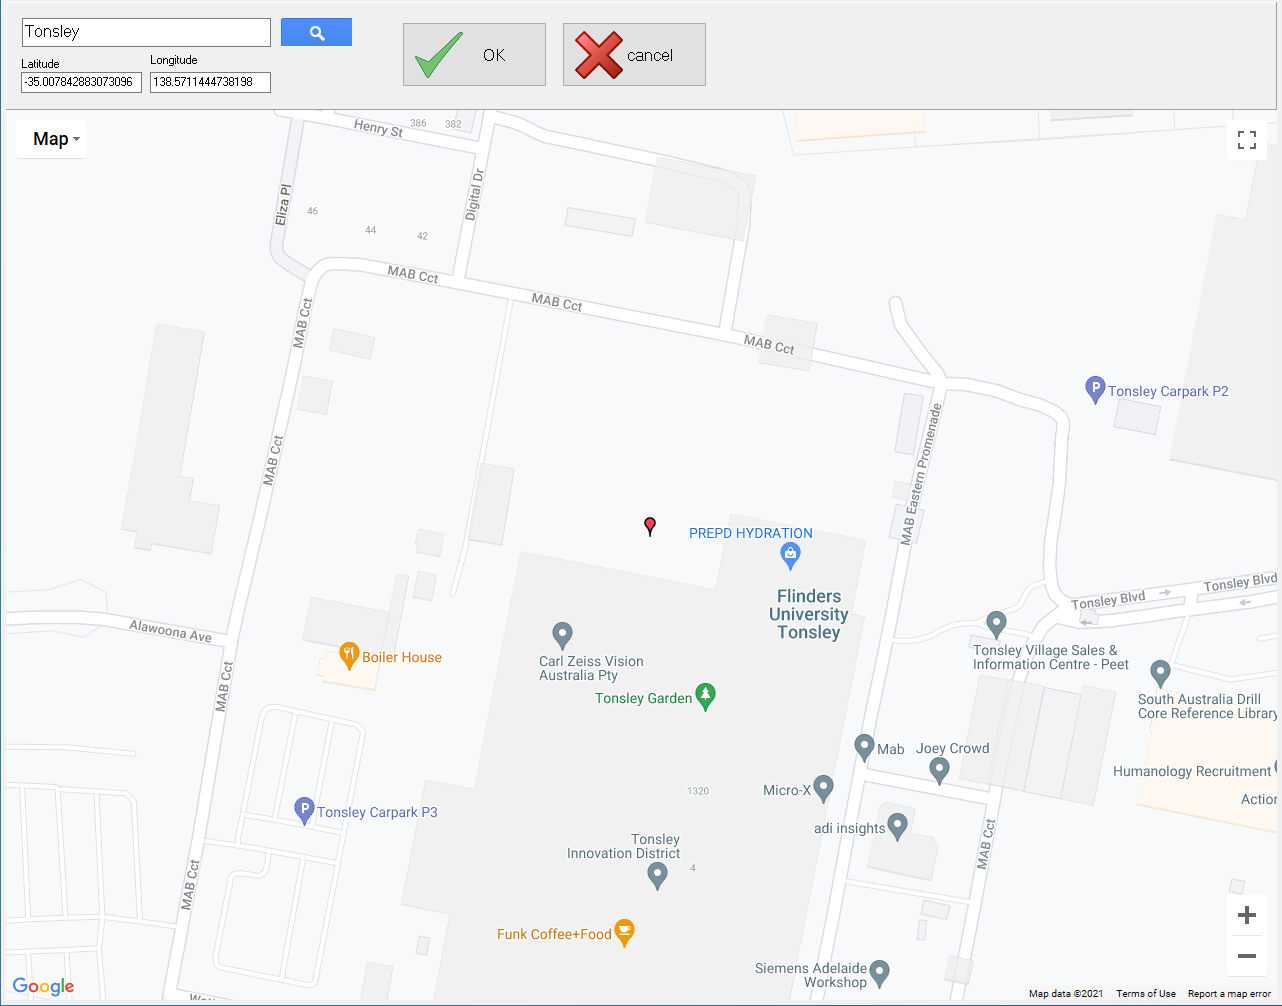
\includegraphics[width=12cm,keepaspectratio]{Figures/static coordinates setup.png}
        \caption{Using google maps within SatGen3 to choose a static coordinate to be used as desired spoof location}
    \label{fig:StaticCoordinate}
    \end{centering}
\end{figure}

\begin{figure}[ht]
    \begin{centering}
        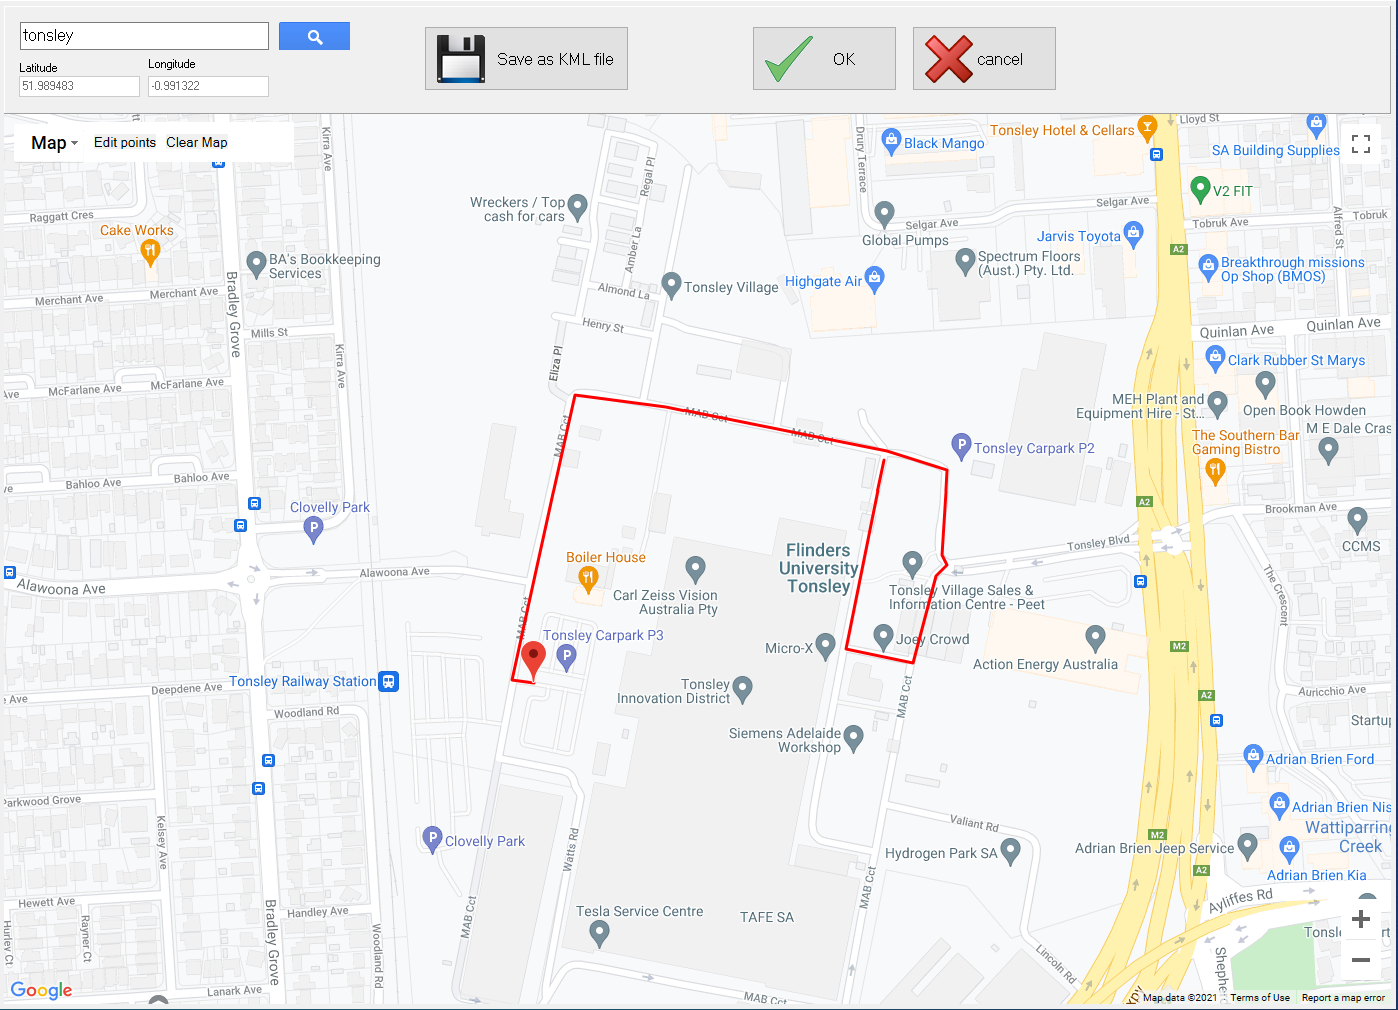
\includegraphics[width=12cm,keepaspectratio]{Figures/dynamic coordinates setup.png}
        \caption{Using google maps within SatGen3 to choose a set of coordiantes to be used as desired spoof path for a dynamic spoof attack}
    \label{fig:DynamicCoordinate}
    \end{centering}
\end{figure}

\subsection{Generate NMEA File}
The coordinate and NMEA file creation step is essentially the same step within the SatGen3 software package. Once the coordinate or path was chosen, it was a matter of
choosing to save the output as a txt file. An example of this is shown in Figure \ref{fig:StaticCoordinateNMEA}.

\begin{figure}[ht]
    \begin{centering}
        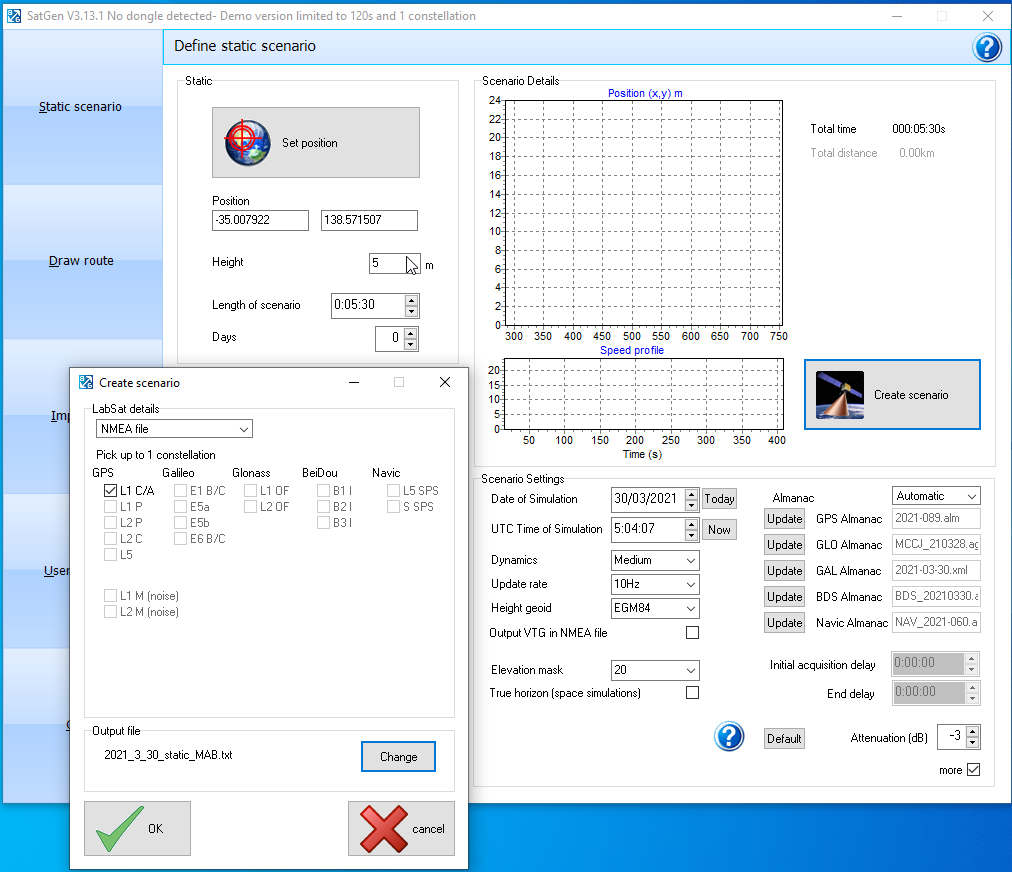
\includegraphics[width=12cm,keepaspectratio]{Figures/2021_03_30_static_MAB_setup.png}
        \caption{Using static coordinate to generate NMEA file}
    \label{fig:StaticCoordinateNMEA}
    \end{centering}
\end{figure}

\subsection{Download Ephemeris}
From the NASA website, hourly versions of the GPS constellation ephemeris, in the form of a RINEX file, are available. These are compiled into a daily file. These daily
files are available all the way from 1992. An account is required to access these files, but there are sample programs provided for retrieving
the files programically using different methods. A script was generated that was able to get the latest version from the website using Python. There were initially some
issues with getting the script to connect to the remote server to gain access to the files. It was found that there was a bug on linux with a certain version of openssl.
A newer version was manually installed and this solved the issue.

The downlaoded file was a compressed version of the text file, and thus it was required to be uncompressed using the tar program.

\subsection{Compile Signal Binary File}
The minimum requirements to compile a binary file using GPS-SDR-SIM was a source coordinate of some sort and the ephemeris for the desired date and time that the spoofer
will transmit. This did not need to match the date and time that the signal was being transmitted on.

Using this information, the place, time and ephemeris the program is able to calcaulate which of the satellites will be in view and what their expected psudo-ranges would
be. The signal modulation is applied wihtin the compilation of the file, simplifying the process of transmitting the file. 

\subsection{Transmit Signal}
Once the signal has been compiled into a binary file it is sent to the USRP SDR via GNURadio. GNURadio has an SDK that allows for text based programming. A script that was
capable of connecting to USRP devices automatically throught he UHD daemon was distributed with the gps-sdr-sim program. This was used to simplify the development
process. 

This was a simple program that connected the source file to the SDR via some simple blocks.

\todo{insert equivelant gnuradio block diagram for program}

An important part of the transmission was that it needed to be performed within a faraday cage for legal purposes. This is discussed in section \ref{sec:FaraCage}.

\subsection{Log GPS Data}
To log the transmitted GPS signals from the SDR a COTS receiver and a smartphone were set up. The COTS receiver has a USB interface that outputs a stream of NMEA
senetences at a 1Hz frequency. This can be modified to 5Hz, but this was not required for these experiments. Using a script the USB port was opened and logged to a text
file. 

When using a smartphone Android was required for logging since the OS allows access to the raw properties of the recveived signal. There is also an intuituve applicaiton
"GNSS Logger" that allows for comprehensive visualistion of current GNSS tracking as well as the ability to log data. This data was logged to a text file using a non
standard layout, but there was an option to log the NMEA sentences as well.  

\subsection{Generate Graphs}
Once there was a log file, graphs were generated to visualise the various parameters of the location resolution as interpretated by the receiver. 
The generation of the graphs that make up the results section was done in python and was based upon the NMEA senetences logged from the receivers. GPS receivers have the
ability to check the validity of signals they recieve. When they are able to resolve a location the value of one of the sentences is changed to reflect this. This was
used to determine the time to first fix of each test. This should not be considered accurate and viewed as an estiamte only.

There is a PC companion application for the GNSS Logger app that allows for comprehensive
graphing and reports to be generated for a particulatr log file.

\section{Using SatGen3}

To generate the binary bitstream for use with an SDR RF front end a GGA NMEA data stream was created using the satgen3 software package. This NMEA stream was used to make
the binary file using the gps-sdr-sim command line interface program. SatGen3 replaces the need for capturing the raw GNSS signals or GGA sentence stream thus increasing
the flexilbilty of scenarios that can be tested. Although there is no guarentee that the simulated stream of information is going to be correct. Thus a capture replay
attack should still be considered as more reliable.

\section{Faraday Cage} \label{sec:FaraCage}
A faraday cage was used for testing purposes for two main reasons. It will isolate the target device from existing legitimate GNSS signals and stop any transmitted
radiation from propagating into the local environment. Isolation from receiving legitimate signals is important since a reciver that is tracking a satellite already is
harder to jam or spoof than one that is not. More important is ensuring that the radiation does not enter the environment since transmitting any signals on the frequency
band for GNSS systems is illegal in Australia. 

Since the received signal strength from a GNSS satellite is so low ($\approx -150dBm$) any signal that is tranmsitted from Earth's surface will be able overpower these
signals for up to 85km, assuming an omnidirectional antenna, as shown in equation \ref{eq:propogationCalc}. This calucation was performed with the assumed maximum
transmission power of the SDR of $15 dBm$ coupled with a $30dB$ attenuator and transmitting on the L1 GPS band. In practise the effective range will be much less due to
attenuation due to objects between transmitter and receiver, but this calculation shows that performing the experiments within a controlled environment was requried.
\begin{equation}    
    \begin{split} \label{eq:propogationCalc}
        Att_{dB} &= 10 \log_{10}\left(\frac{c}{4\pi df}\right)^2 \\
        d = \frac{c}{4\pi 10^{\left(\frac{Att_{dB}}{20}\right)}f} &= \frac{3\times10^8}{4\pi 10^{-6.75}1.57542\times 10^9} \approx 85km
    \end{split}
\end{equation}

\section{Experimental Issues}
While performing experiments there were issues thaat were run into that were required to be overcome. Initially a Log Periodic antenna was used for transmission since its
frequency range was appropriate for use transmitting L1 band signals. After experiments failed to pick up any signals it was swapped for a omnidirectional antenna. This
was able to produce signals that were picked up by the GNSSLogger application. Observing the graphs of the carrier to noise figure showed that when there was an underrun
issue the $\frac{C}{N_0}$ would drop to 0 and the GPS receiver in the phone would lose connection to the 'satellites'. This meant that no GPS lock was achievable.  

In an attempt to overcome the underrun issue that was plagueing the experiments, a new PC was brought in with Ubuntu installed directly instead of via a VM. This resulted
in the radio working straight away. The underrun issues resurfaced when trying to read the serial data from a COTS gps receiver. This was less than ideal and required a
second computer to act as a datalogger.

\section{Experiments}
Experimentation was performed at the Tonsley campus of Flinders University, which has GPS coordinates of $-35.007650, 138.572030$. At first it was decided to use the
centre of the Adelaide CBD as the coordinates for spoofing, that is $-34.5571732282, 138.3599516878$. Therefore it would be considered successful if the gps receiver was to show
that the current locaiton was in the CBD.

\subsection{Hardware Setup}
For all experiments the same hardware was used. This included the USRP SDR, laptop and GPS receiver. The laptop was an important piece of eqiupment since it needed to be
powerful enough to be able to feed the data to the SDR quick enough to avoid the aformentioned underrun issues. Towards the end of the project there was a hardware fault
with the Pixel XL phone receiver. This was replaced by the Pixel 4a 5G.

There was no formal decision process for choosing the hardware components since they were all parts that had already been purchased and were in possesion of the
supurvisor. Having said that some research went into the suitabilty of the equipment, mainly the SDR. It was found that this was one of the most powerful and most
importantly had one of the most stable clock osiclators availble in software defined radios. This made is well suited to GNSS based tasks. Alternatives, like the
RTL-SDR are capable devices for the cost, but only offer reception. Duplex options like the HackRF are also suitable for transmitting high bandwidth signals, however the
on board clock is not stable enough for highly accurate signals like that of GNSS. There was a workaround for this, which included desoldering the included oscillator and
soldering a more stable part. In future, if access to USRP based SDR's is not availble then this would be a very good second option. However, there was access to a better
tool, being the N210, therfore it was chosen. From Ettus, there were two daughtercards that allow access to the desired 1575.42MHz band of the L1 GPS signal, the SBX and
WBX. The SBX was chosen because it was already available. It should be noted that there would be no theoretical difference between either daughtercard since the desired
freqeuency was not at the extreme of either cards bands.

\begin{itemize}
    \item Laptop
    \begin{itemize}
        \item Dell Inspiron 15
        \item CPU: Core i7 Quad Core/ 8 thread
        \item RAM: 32GB
        \item Ethernet Connection: gigabit
    \end{itemize}
    \item Software defined radio
    \begin{itemize}
        \item USRP N210
        \item SBX-40 daughtercard
        \item 30dB attenuator
        \item Full duplex
        \item Gigbit Ethernet connection
        \item high performace FPGA
        \item omnidirection antenna
    \end{itemize}
    \item GPS Receiver (Phone 1)
    \begin{itemize}
        \item Google Pixel XL
        \item Android 10
        \item Multi constellation GNSS support (GPS+QZSS, GLONASS, Beidou)
    \end{itemize}
    \item GPS Receiver (Phone 2)
    \begin{itemize}
        \item Google Pixel 4a 5G
        \item Android 11
        \item Multi constellation GNSS support (GPS+QZSS, GLONASS, Beidou)
    \end{itemize}
    \item GPS Receiver (COTS)
    \begin{itemize}
        \item GPS L1 support only
        \item NMEA output
    \end{itemize}
\end{itemize}

\begin{figure}[h]
    \begin{centering}
        \includegraphics[width=13cm,keepaspectratio]{Figures/Setup/overview_labelled.png}
        \caption{Hardware setup for testing spoofing transmission within Faraday cage}
    \label{fig:HardwareSetup}
    \end{centering}
\end{figure}

\subsection{Software Setup}
The laptop was the interface between softrware and hardware. It was used to generate the binary files and then to control the SDR. The SDR would not operate without the
PC attached to the ethernet port.

The software used for this project was a combination of open source and custom software. 
The software was chosen while performing the literature review. There were examples \emph{\textbf{Insert citations that used gps-sdr-sim}} of using open source programs
for the purpose of GPS spoofing. This was the best step forward since there were credible results with that software.

Custom software was created for the reporting and results of the experiments. 

\begin{itemize}
    \item GPS-SDR-sim
    \item GNURadio
\end{itemize}

\subsection{Static Spoofing}
Within this thesis static spoofing is defined as producing a signal that produces a calculated location that does not change over time. While in practise there was some
minor movement caused by the uncertainty in trilateration, this change in position is minor and within the range of error of GPS positioning.
Using the SatGen3 software a location was chosen as the spoof location. After setting the desired time and date of spoofing the scenario was created. THis 

\subsection{Dynamic Spoofing}
Dynamic spoofing refers to the production of a signal that when used to calcluate position, will be shown to change over time. The path traced by the receiver will be
set at the time of production of the binary file, see figure \ref{fig:21MarCBDDynamic}, but there will be perceived motion.

\subsection{Real-Time Spoofing}
Due to time constraints a real-time algorithm was not produced as part of this project. However, utelising the open source projects that have been used to complete this
thesis it would be probable to be able to create a real time spoofing device that would be able to react to the positional changes of the receiver instead of following a
pre-determined path when generating the binary file. The signals generation algorithm could be ported to a GNURadio block in C++ to allow for easy access to real-time GPS
signal spoofing. If an SDR is a full duplex radio, such is the case for the USRP N210, then one port can be receiveing the real GNSS signal and the other can be
transmitting the spoofed signal. Care would need to be taken in the set up of this arrangement since any transmitted signal would also be picked up by the reciving
antenna. Therefore a directional transmitting antenna and physical disctance should be employed to allow for legitimate GNSS signals to reach the reciever port. 

\section{Parameters required for successful spoofing}
\todo{add screen shots of steps required to generate binary file}
Due to the internal workings of the USRP, there needs to be an integer ratio between the clock rate and sample rate. Therefore is was required that the sample frequency
was set to 2.5Msps instead of the default 2.6Msps that the software would normally use.

\begin{figure}[h]
    \begin{centering}
        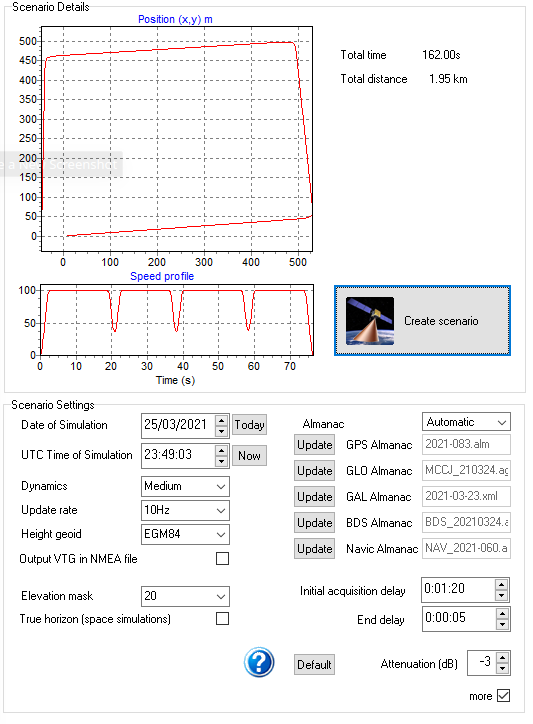
\includegraphics[width=10cm,height=10cm,keepaspectratio]{Figures/21-3-25_cbd_dynamic_setup.png}
        \caption{Settings of SatGen3 used to generate the dynamic path loop around Adelaide CBD. There is a graph that shows the offset from the origin and speed aver the journey}
    \label{fig:21MarCBDDynamic}
    \end{centering}
\end{figure}

\section{SDR Setup for GNSS Reception}
Reception of GNSS signals is a compliated process which involves sychronising time values and solving simultaneous equtations for position, therefore it was decided that
the opensource program GNSS-SDR would be used to perform all of these functions. This sofware has been built over a number of years and is able to receive different GNSS
signals and translate them into position.

The hardware setup for this was different. Since the signal strength of a GNSS transmission is so low when it reaches the earths surface ($\approx -160dBm$) an active
antenna is typically requied for best performance, especially if there is no clear view of the sky or if there are many buildings that add multipath signals into
consideration.
